% =====================================================================
%  IRexp / Scientific Data -- Figure 3: composition and validation
%  Panels a-f (lowercase, matching the manuscript caption).
%  Canvas 183 mm (Nature double column) x 198 mm.
%  Agent OPUS. Every count comes from ../../tikz/frozen_plot_data.json;
%  the coordinate blocks below are transcribed from that file verbatim.
%
%  Panels a, b, c, e are hand-set horizontal bars: they carry no x axis
%  at all (direct value labels only), which is cheaper and more precise
%  in raw TikZ than an axis with every tick suppressed.  Panels d and f
%  are real pgfplots axes because they need ticks and gridlines.
% =====================================================================
\documentclass[border=0pt,tikz]{standalone}

\usepackage[T1]{fontenc}      % proper dashes, quotes and \textbullet from the text font
\usepackage{textcomp}         % \texttimes etc. from TS1 Nimbus Sans, not Computer Modern
\makeatletter\@namedef{ver@sansmathfonts.sty}{2023/01/01}\makeatother
% Nature Portfolio / Scientific Data shared TikZ style for IRexp figures.
% Width: 183 mm double-column. Typography: Helvetica-class (phv).
\RequirePackage{tikz}
\RequirePackage{pgfplots}
\RequirePackage{xcolor}
\RequirePackage{helvet}
\IfFileExists{sansmathfonts.sty}{\RequirePackage{sansmathfonts}}{}
\renewcommand{\familydefault}{\sfdefault}
\pgfplotsset{compat=1.18}
\usetikzlibrary{
  arrows.meta,calc,positioning,fit,shapes.geometric,shapes.misc,
  backgrounds,shadows.blur,patterns,decorations.pathreplacing
}

% ---- Paul Tol / NMRexp-matched palette ----
\definecolor{nmrBlue}{HTML}{4A7EBB}
\definecolor{nmrBlueDark}{HTML}{2E5F8F}
\definecolor{nmrBlueLight}{HTML}{A8C8E8}
\definecolor{nmrPeach}{HTML}{E8B48C}
\definecolor{nmrNavy}{HTML}{1B3D5C}
\definecolor{nmrRed}{HTML}{C44E52}
\definecolor{nmrGreen}{HTML}{3D8B5E}
\definecolor{nmrOrange}{HTML}{D97B32}
\definecolor{ink}{HTML}{1A1A1A}
\definecolor{muted}{HTML}{7A7F85}
\definecolor{note}{HTML}{5C636A}
\definecolor{faint}{HTML}{E8EAEC}
\definecolor{ghost}{HTML}{C5C9CD}
\definecolor{tintBlue}{HTML}{EEF3F8}
\definecolor{tintGreen}{HTML}{EAF4EE}

\newcommand{\NatureFont}{\fontfamily{phv}\selectfont}
\newcommand{\PanelLabel}[1]{%
  {\NatureFont\bfseries\fontsize{8}{9.6}\selectfont #1}%
}
\newcommand{\FigBody}{\NatureFont\fontsize{7}{8.4}\selectfont}
\newcommand{\FigSmall}{\NatureFont\fontsize{5.5}{6.6}\selectfont}
\newcommand{\FigAxis}{\NatureFont\fontsize{7}{8.4}\selectfont}

\tikzset{
  nature arrow/.style={
    -{Latex[length=1.6mm,width=1.3mm]},
    line width=0.55pt, ink
  },
  nature arrow grey/.style={
    -{Latex[length=1.6mm,width=1.3mm]},
    line width=0.5pt, note
  },
  stage card/.style={
    draw=nmrBlueDark, line width=0.7pt, rounded corners=2.2pt,
    fill=white, inner sep=3pt, align=center, font=\FigBody
  },
  stage header/.style={
    fill=nmrBlueDark, text=white, font=\FigBody\bfseries,
    rounded corners=2.2pt, inner sep=2.5pt, align=center
  },
  soft card/.style={
    draw=ghost, line width=0.55pt, rounded corners=2.2pt,
    fill=white, inner sep=3.5pt, align=left, font=\FigBody
  },
}

\pgfplotsset{
  nature axis/.style={
    tick label style={font=\FigSmall, /pgf/number format/assume math mode},
    label style={font=\FigAxis\bfseries},
    title style={font=\FigBody\bfseries, color=ink},
    axis line style={ink, line width=0.5pt},
    tick style={ink, line width=0.45pt},
    major grid style={faint, line width=0.35pt},
    axis x line=bottom,
    axis y line=left,
    enlarge x limits=false,
    clip=false,
  },
  nature hbar/.style={
    nature axis,
    xbar,
    bar width=7pt,
    y=data,
    nodes near coords,
    every node near coord/.append style={
      font=\FigSmall, ink, anchor=west, /pgf/number format/fixed,
      /pgf/number format/1000 sep={,}
    },
    xtick=\empty,
    axis x line=none,
    y axis line style={ink, line width=0.55pt},
    ytick style={draw=none},
    y tick label style={font=\FigBody, ink, anchor=east},
    grid=major x,
    xmin=0,
  },
}

\renewcommand{\familydefault}{\sfdefault}
\usepackage[helvet]{sfmath}

\newcommand{\FigTiny}{\NatureFont\fontsize{5}{6}\selectfont}

% ---------------------------------------------------------------------
%  Horizontal-bar helper.  \Sx spine, \Sw field width, \Sm field maximum
%  (in thousands of records); redefined before each panel.
% ---------------------------------------------------------------------
\def\Sx{23}\def\Sw{21}\def\Sm{121.233}
% {row y}{value/1000}{bar height}{fill}{category label}{value label}
\newcommand{\HRow}[6]{%
  \pgfmathsetmacro{\blen}{#2*\Sw/\Sm}%
  \draw[faint,line width=0.3pt] (\Sx,#1) -- ({\Sx+\Sw},#1);
  \fill[#4] (\Sx,{#1-#3/2}) rectangle ({\Sx+\blen},{#1+#3/2});
  \node[anchor=east,inner sep=0pt,text=ink,font=\FigBody] at ({\Sx-1.4},#1) {#5};
  \node[anchor=west,inner sep=0pt,text=ink,font=\FigSmall] at ({\Sx+\blen+1.1},#1) {#6};%
}
% Panel head: {letter}{x}{title}{subtitle}
\newcommand{\PanelHead}[4]{%
  \node[anchor=north west,inner sep=0pt] at (#2,197) {\PanelLabel{#1}};
  \node[anchor=base west,inner sep=0pt,text=ink,font=\FigBody] at ({#2+5.2},194)
    {\bfseries #3};
  \node[anchor=base west,inner sep=0pt,text=note,font=\FigSmall] at ({#2+5.2},191)
    {#4};%
}
% Element row: {row y}{value/1000}{label}{value label}
\newcommand{\ERow}[4]{%
  \pgfmathsetmacro{\blen}{#2*\Sw/\Sm}%
  \draw[faint,line width=0.3pt] (\Sx,#1) -- ({\Sx+\Sw},#1);
  \fill[nmrBlue] (\Sx,{#1-1.4}) rectangle ({\Sx+\blen},{#1+1.4});
  \node[anchor=east,inner sep=0pt,text=ink,font=\FigBody] at ({\Sx-1.4},#1) {#3};
  \node[anchor=west,inner sep=0pt,text=ink,font=\FigSmall] at ({\Sx+\blen+1.1},#1) {#4};%
}

\pgfplotsset{
  irexp hist/.style={
    nature axis,
    scale only axis,
    ymajorgrids=true,
    xmajorgrids=false,
    ymin=0,
    axis x line*=bottom,          % starred: no arrow tips, Nature house style
    axis y line*=left,
    axis line style={ink,line width=0.5pt,-},
    scaled y ticks=false,
    yticklabel style={/pgf/number format/fixed,/pgf/number format/1000 sep={,}},
    % With `axis x line=bottom` pgfplots offsets the axis labels from the
    % axis LINE, not from the tick labels, so a centred xlabel lands on top
    % of the middle tick.  `near ticks` measures from the tick label box
    % instead -- but it *replaces* the label style, so the two `label style`
    % keys below have to come after it or the font reverts to 10 pt.
    xlabel near ticks,
    ylabel near ticks,
    xlabel shift=2.6pt,          % `near ticks` leaves zero clearance
    ylabel shift=1.6pt,
    x label style={font=\FigSmall,color=ink},
    y label style={font=\FigSmall,color=ink},
    tick align=outside,
  },
  % Panel d: 20 adjacent bins, so a hairline outline acts as a bin divider.
  irexp bars/.style={
    ybar interval, fill=nmrBlue, draw=nmrBlueDark, line width=0.25pt,
  },
  % Panel f: the distributions are spiky and most bins are empty.  An
  % outline would draw a stray rule along the axis through every empty
  % bin, so these bars are fill-only; single-record bins still resolve
  % because each sub-panel is 22 mm tall.
  irexp bars flat/.style={
    ybar interval, fill=nmrBlue, draw=none,
  },
}

% A pgfplots axis cannot be placed with `at=` inside a picture whose unit
% vectors are millimetres, so each axis lives in its own nested picture
% whose bounding box is pinned to the plot rectangle.  The wrapper then
% anchors that rectangle exactly: \PlotBox{x}{y}{axis code}.
\newcommand{\PlotBox}[3]{%
  \node[anchor=south west,inner sep=0pt] at (#1,#2) {\begin{tikzpicture}#3%
    \pgfresetboundingbox
    \useasboundingbox (ax.south west) rectangle (ax.north east);
  \end{tikzpicture}};%
}

\begin{document}\NatureFont
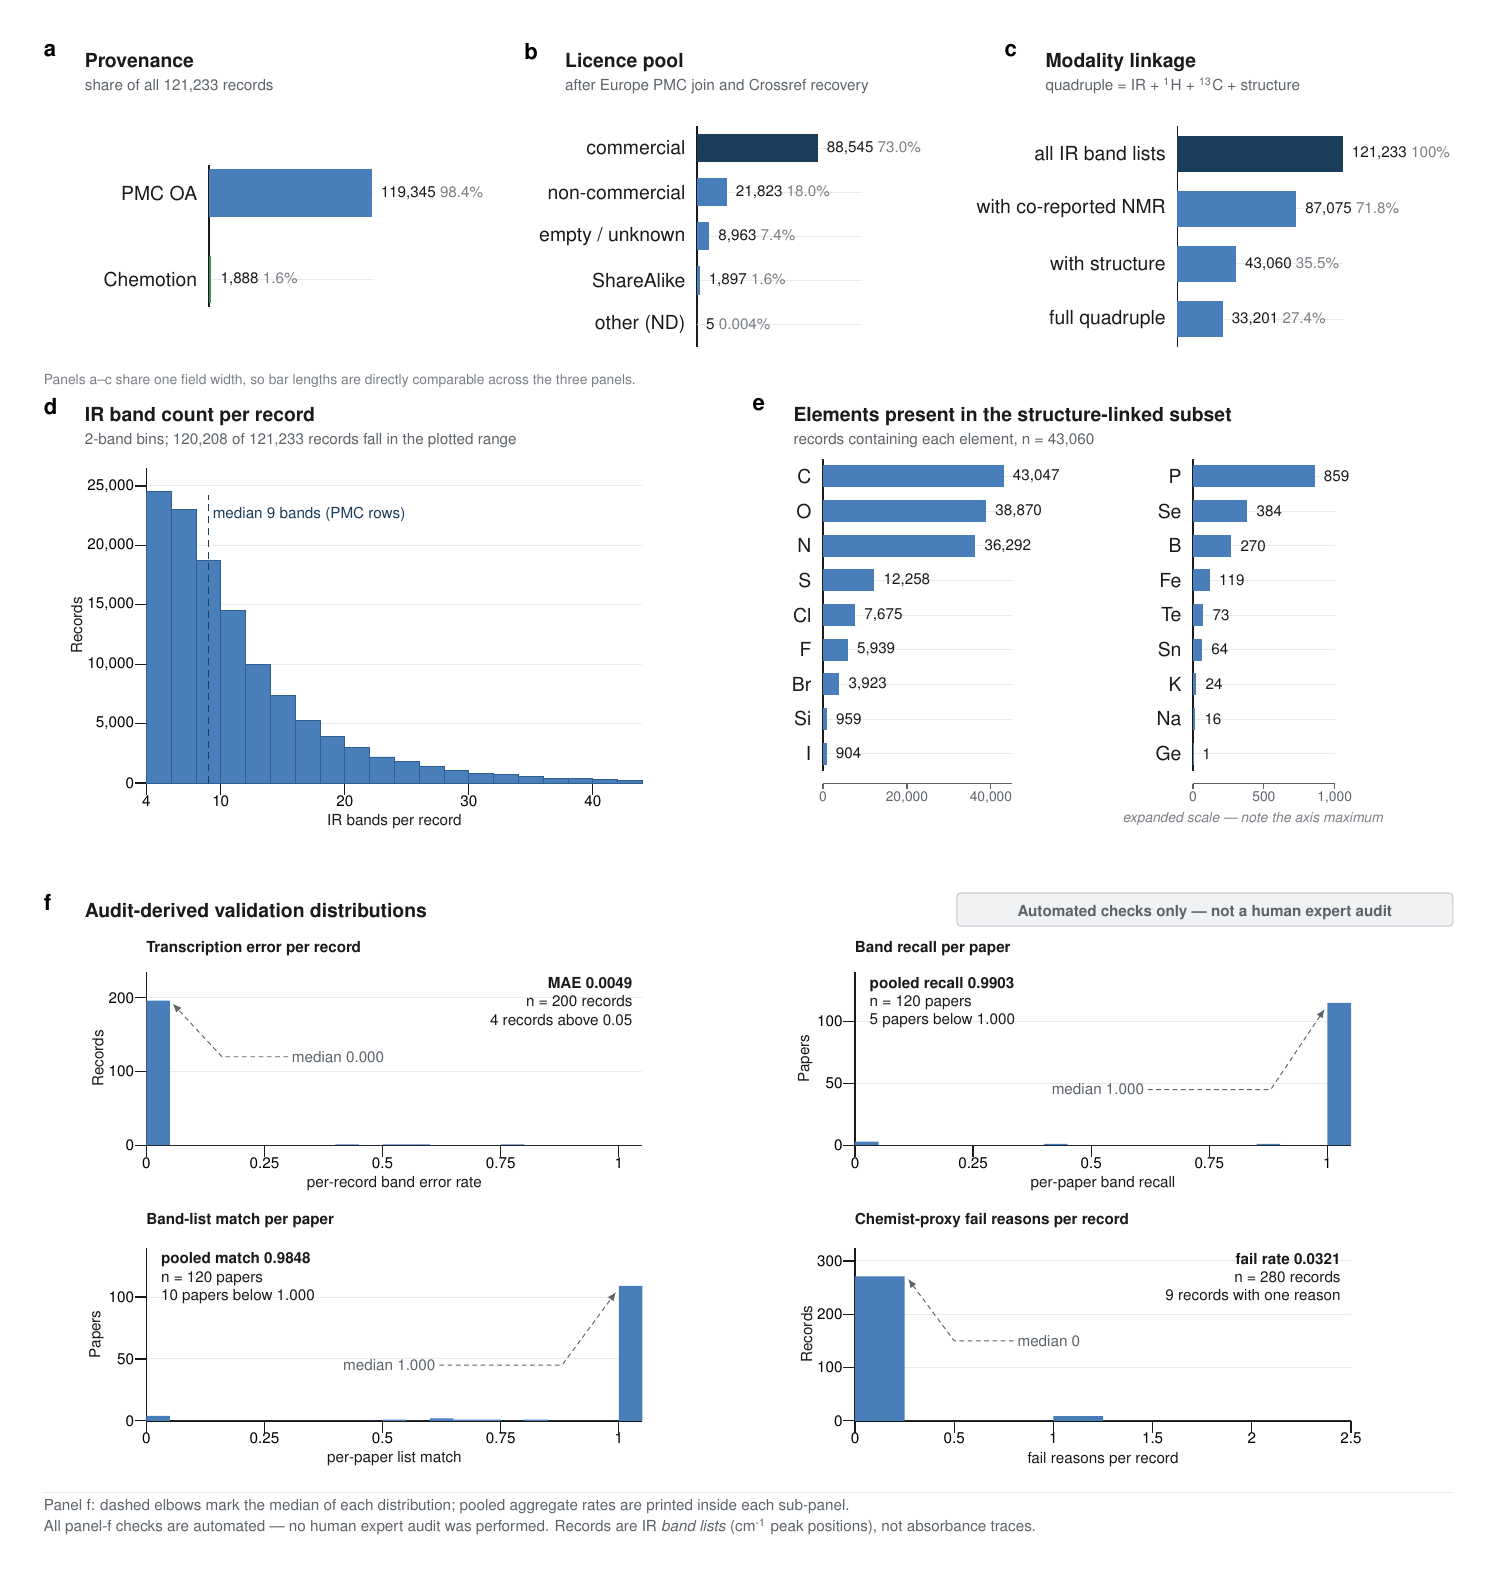
\begin{tikzpicture}[x=1mm,y=1mm,line cap=butt]
\useasboundingbox (0,5.5) rectangle (183,199);

% =====================================================================
%  ROW 1 -- panels a, b, c : composition, one shared 0-121,233 field
% =====================================================================

% --- a  Provenance ---------------------------------------------------
\PanelHead{a}{2}{Provenance}{share of all 121,233 records}
\def\Sx{23}\def\Sw{21}\def\Sm{121.233}
% Two rows only, so the spine hugs them and the whole group is optically
% centred on the taller spines of b and c rather than dangling below them.
\draw[ink,line width=0.55pt] (\Sx,163.5) -- (\Sx,181.5);
\HRow{178.0}{119.345}{6.0}{nmrBlue}{PMC OA}{119,345\ \textcolor{muted}{98.4\%}}
\HRow{167.0}{1.888}{6.0}{nmrGreen}{Chemotion}{1,888\ \textcolor{muted}{1.6\%}}

% --- b  Licence pool -------------------------------------------------
\PanelHead{b}{63}{Licence pool}{after Europe PMC join and Crossref recovery}
\def\Sx{85}\def\Sw{21}\def\Sm{121.233}
\draw[ink,line width=0.55pt] (\Sx,158.5) -- (\Sx,186.5);
\HRow{183.7}{88.545}{3.6}{nmrNavy}{commercial}{88,545\ \textcolor{muted}{73.0\%}}
\HRow{178.1}{21.823}{3.6}{nmrBlue}{non-commercial}{21,823\ \textcolor{muted}{18.0\%}}
\HRow{172.5}{8.963}{3.6}{nmrBlue}{empty / unknown}{8,963\ \textcolor{muted}{7.4\%}}
\HRow{166.9}{1.897}{3.6}{nmrBlue}{ShareAlike}{1,897\ \textcolor{muted}{1.6\%}}
\HRow{161.3}{0.005}{3.6}{nmrBlue}{other (ND)}{5\ \textcolor{muted}{0.004\%}}

% --- c  Modality linkage ---------------------------------------------
\PanelHead{c}{124}{Modality linkage}{quadruple $=$ IR $+$ \textsuperscript{1}H $+$ \textsuperscript{13}C $+$ structure}
\def\Sx{146}\def\Sw{21}\def\Sm{121.233}
\draw[ink,line width=0.55pt] (\Sx,158.5) -- (\Sx,186.5);
\HRow{183.0}{121.233}{4.6}{nmrNavy}{all IR band lists}{121,233\ \textcolor{muted}{100\%}}
\HRow{176.0}{87.075}{4.6}{nmrBlue}{with co-reported NMR}{87,075\ \textcolor{muted}{71.8\%}}
\HRow{169.0}{43.060}{4.6}{nmrBlue}{with structure}{43,060\ \textcolor{muted}{35.5\%}}
\HRow{162.0}{33.201}{4.6}{nmrBlue}{full quadruple}{33,201\ \textcolor{muted}{27.4\%}}

\node[anchor=north west,inner sep=0pt,text=muted,font=\FigTiny] at (2,155)
  {Panels a--c share one field width, so bar lengths are directly comparable across the three panels.};

% =====================================================================
%  ROW 2 -- panel d : band-count histogram
% =====================================================================
\node[anchor=north west,inner sep=0pt] at (2,152) {\PanelLabel{d}};
\node[anchor=base west,inner sep=0pt,text=ink,font=\FigBody] at (7.2,149)
  {\bfseries IR band count per record};
\node[anchor=base west,inner sep=0pt,text=note,font=\FigSmall] at (7.2,146)
  {2-band bins; 120,208 of 121,233 records fall in the plotted range};

\PlotBox{15}{103}{%
\begin{axis}[
  irexp hist, name=ax, width=63mm, height=40mm,
  xmin=4, xmax=44, ymax=26500,
  xtick={4,10,20,30,40},
  ytick={0,5000,10000,15000,20000,25000},
  xlabel={IR bands per record},
  ylabel={Records},
]
  \addplot[irexp bars] coordinates {
    (4,24556) (6,22989) (8,18726) (10,14534) (12,9959) (14,7368)
    (16,5241) (18,3899) (20,3017) (22,2202) (24,1822) (26,1426)
    (28,1069) (30,826) (32,698) (34,534) (36,386) (38,408)
    (40,298) (42,250) (44,0)
  };
  \draw[nmrNavy,line width=0.5pt,dash pattern=on 0.9mm off 0.6mm]
    (axis cs:9,0) -- (axis cs:9,24200);
  \node[anchor=west,inner sep=1.4pt,text=nmrNavy,font=\FigSmall] at (axis cs:9,22600)
    {median 9 bands (PMC rows)};
\end{axis}}

% =====================================================================
%  ROW 2 -- panel e : elemental composition, two columns
% =====================================================================
\node[anchor=north west,inner sep=0pt] at (92,152) {\PanelLabel{e}};
\node[anchor=base west,inner sep=0pt,text=ink,font=\FigBody] at (97.2,149)
  {\bfseries Elements present in the structure-linked subset};
\node[anchor=base west,inner sep=0pt,text=note,font=\FigSmall] at (97.2,146)
  {records containing each element, n $=$ 43,060};

% left column: nine most frequent, field scaled to 45,000
\def\Sx{101}\def\Sw{24}\def\Sm{45}
\draw[ink,line width=0.55pt] (\Sx,104.6) -- (\Sx,144.2);
\ERow{142.0}{43.047}{C}{43,047}
\ERow{137.6}{38.870}{O}{38,870}
\ERow{133.2}{36.292}{N}{36,292}
\ERow{128.8}{12.258}{S}{12,258}
\ERow{124.4}{7.675}{Cl}{7,675}
\ERow{120.0}{5.939}{F}{5,939}
\ERow{115.6}{3.923}{Br}{3,923}
\ERow{111.2}{0.959}{Si}{959}
\ERow{106.8}{0.904}{I}{904}
\pgfmathsetmacro{\eaT}{101+20*24/45}
\pgfmathsetmacro{\ebT}{101+40*24/45}
\draw[note,line width=0.4pt] (101,103.0) -- (125,103.0);
\foreach \tx in {101,\eaT,\ebT}{\draw[note,line width=0.4pt] (\tx,103.0) -- (\tx,102.3);}
\node[anchor=north,inner sep=0pt,text=note,font=\FigTiny] at (101,102.0) {0};
\node[anchor=north,inner sep=0pt,text=note,font=\FigTiny] at (\eaT,102.0) {20,000};
\node[anchor=north,inner sep=0pt,text=note,font=\FigTiny] at (\ebT,102.0) {40,000};

% right column: nine remaining, field expanded to 1,000
\def\Sx{148}\def\Sw{18}\def\Sm{1}
\draw[ink,line width=0.55pt] (\Sx,104.6) -- (\Sx,144.2);
\ERow{142.0}{0.859}{P}{859}
\ERow{137.6}{0.384}{Se}{384}
\ERow{133.2}{0.270}{B}{270}
\ERow{128.8}{0.119}{Fe}{119}
\ERow{124.4}{0.073}{Te}{73}
\ERow{120.0}{0.064}{Sn}{64}
\ERow{115.6}{0.024}{K}{24}
\ERow{111.2}{0.016}{Na}{16}
\ERow{106.8}{0.001}{Ge}{1}
\draw[note,line width=0.4pt] (148,103.0) -- (166,103.0);
\foreach \tx in {148,157,166}{\draw[note,line width=0.4pt] (\tx,103.0) -- (\tx,102.3);}
\node[anchor=north,inner sep=0pt,text=note,font=\FigTiny] at (148,102.0) {0};
\node[anchor=north,inner sep=0pt,text=note,font=\FigTiny] at (157,102.0) {500};
\node[anchor=north,inner sep=0pt,text=note,font=\FigTiny] at (166,102.0) {1,000};
\node[anchor=north west,inner sep=0pt,text=muted,font=\FigTiny] at (139,99.4)
  {\itshape expanded scale --- note the axis maximum};

% =====================================================================
%  ROW 3 -- panel f : automated validation distributions
% =====================================================================
\node[anchor=north west,inner sep=0pt] at (2,89) {\PanelLabel{f}};
\node[anchor=base west,inner sep=0pt,text=ink,font=\FigBody] at (7.2,86)
  {\bfseries Audit-derived validation distributions};
\draw[ghost,line width=0.4pt,rounded corners=1.4pt,fill=faint!60!white]
  (118,84.9) rectangle (181,89.1);
\node[anchor=center,inner sep=0pt,text=note,font=\FigSmall] at (149.5,86.6)
  {\bfseries Automated checks only --- not a human expert audit};

% --- f1 transcription error ------------------------------------------
\node[anchor=base west,inner sep=0pt,text=ink,font=\FigSmall] at (15,81.5)
  {\bfseries Transcription error per record};
\PlotBox{15}{57}{%
\begin{axis}[
  irexp hist, name=ax, width=63mm, height=22mm,
  xmin=0, xmax=1.05, ymax=235,
  xtick={0,0.25,0.5,0.75,1}, ytick={0,100,200},
  xlabel={per-record band error rate}, ylabel={Records},
]
  \addplot[irexp bars flat] coordinates {
    (0,196) (0.05,0) (0.1,0) (0.15,0) (0.2,0) (0.25,0) (0.3,0)
    (0.35,0) (0.4,1) (0.45,0) (0.5,1) (0.55,1) (0.6,0) (0.65,0)
    (0.7,0) (0.75,1) (0.8,0) (0.85,0) (0.9,0) (0.95,0) (1,0)
    (1.05,0)
  };
  \draw[note,line width=0.35pt,dash pattern=on 0.6mm off 0.45mm,
        -{Latex[length=1.1mm,width=0.9mm]}]
    (axis cs:0.30,120) -- (axis cs:0.16,120) -- (axis cs:0.056,192);
  \node[anchor=west,inner sep=1.2pt,text=note,font=\FigSmall] at (axis cs:0.30,120)
    {median 0.000};
  \node[anchor=north east,align=right,inner sep=0pt,text=ink,font=\FigSmall,inner ysep=0pt]
    at (axis cs:1.03,228) {\textbf{MAE 0.0049}\\n $=$ 200 records\\4 records above 0.05};
\end{axis}}

% --- f2 band recall per paper ----------------------------------------
\node[anchor=base west,inner sep=0pt,text=ink,font=\FigSmall] at (105,81.5)
  {\bfseries Band recall per paper};
\PlotBox{105}{57}{%
\begin{axis}[
  irexp hist, name=ax, width=63mm, height=22mm,
  xmin=0, xmax=1.05, ymax=140,
  xtick={0,0.25,0.5,0.75,1}, ytick={0,50,100},
  xlabel={per-paper band recall}, ylabel={Papers},
]
  \addplot[irexp bars flat] coordinates {
    (0,3) (0.05,0) (0.1,0) (0.15,0) (0.2,0) (0.25,0) (0.3,0)
    (0.35,0) (0.4,1) (0.45,0) (0.5,0) (0.55,0) (0.6,0) (0.65,0)
    (0.7,0) (0.75,0) (0.8,0) (0.85,1) (0.9,0) (0.95,0) (1,115)
    (1.05,0)
  };
  \draw[note,line width=0.35pt,dash pattern=on 0.6mm off 0.45mm,
        -{Latex[length=1.1mm,width=0.9mm]}]
    (axis cs:0.62,45) -- (axis cs:0.88,45) -- (axis cs:0.994,110);
  \node[anchor=east,inner sep=1.2pt,text=note,font=\FigSmall] at (axis cs:0.62,45)
    {median 1.000};
  \node[anchor=north west,align=left,inner sep=0pt,text=ink,font=\FigSmall,inner ysep=0pt]
    at (axis cs:0.03,136) {\textbf{pooled recall 0.9903}\\n $=$ 120 papers\\5 papers below 1.000};
\end{axis}}

% --- f3 list match per paper -----------------------------------------
\node[anchor=base west,inner sep=0pt,text=ink,font=\FigSmall] at (15,47)
  {\bfseries Band-list match per paper};
\PlotBox{15}{22}{%
\begin{axis}[
  irexp hist, name=ax, width=63mm, height=22mm,
  xmin=0, xmax=1.05, ymax=140,
  xtick={0,0.25,0.5,0.75,1}, ytick={0,50,100},
  xlabel={per-paper list match}, ylabel={Papers},
]
  \addplot[irexp bars flat] coordinates {
    (0,4) (0.05,0) (0.1,0) (0.15,0) (0.2,0) (0.25,0) (0.3,0)
    (0.35,0) (0.4,0) (0.45,0) (0.5,1) (0.55,0) (0.6,2) (0.65,1)
    (0.7,1) (0.75,0) (0.8,1) (0.85,0) (0.9,0) (0.95,0) (1,109)
    (1.05,0)
  };
  \draw[note,line width=0.35pt,dash pattern=on 0.6mm off 0.45mm,
        -{Latex[length=1.1mm,width=0.9mm]}]
    (axis cs:0.62,45) -- (axis cs:0.88,45) -- (axis cs:0.994,104);
  \node[anchor=east,inner sep=1.2pt,text=note,font=\FigSmall] at (axis cs:0.62,45)
    {median 1.000};
  \node[anchor=north west,align=left,inner sep=0pt,text=ink,font=\FigSmall,inner ysep=0pt]
    at (axis cs:0.03,136) {\textbf{pooled match 0.9848}\\n $=$ 120 papers\\10 papers below 1.000};
\end{axis}}

% --- f4 chemist-proxy fail reasons -----------------------------------
\node[anchor=base west,inner sep=0pt,text=ink,font=\FigSmall] at (105,47)
  {\bfseries Chemist-proxy fail reasons per record};
\PlotBox{105}{22}{%
\begin{axis}[
  irexp hist, name=ax, width=63mm, height=22mm,
  xmin=0, xmax=2.5, ymax=325,
  xtick={0,0.5,1,1.5,2,2.5}, ytick={0,100,200,300},
  xlabel={fail reasons per record}, ylabel={Records},
]
  \addplot[irexp bars flat] coordinates {
    (0,271) (0.25,0) (0.5,0) (0.75,0) (1,9) (1.25,0) (1.5,0)
    (1.75,0) (2,0) (2.25,0) (2.5,0)
  };
  \draw[note,line width=0.35pt,dash pattern=on 0.6mm off 0.45mm,
        -{Latex[length=1.1mm,width=0.9mm]}]
    (axis cs:0.80,150) -- (axis cs:0.50,150) -- (axis cs:0.268,266);
  \node[anchor=west,inner sep=1.2pt,text=note,font=\FigSmall] at (axis cs:0.80,150)
    {median 0};
  \node[anchor=north east,align=right,inner sep=0pt,text=ink,font=\FigSmall,inner ysep=0pt]
    at (axis cs:2.45,316) {\textbf{fail rate 0.0321}\\n $=$ 280 records\\9 records with one reason};
\end{axis}}

% =====================================================================
%  Footnote
% =====================================================================
\draw[faint,line width=0.4pt] (2,13.0) -- (181,13.0);
\node[anchor=north west,inner sep=0pt,text=note,font=\FigSmall,align=left,inner ysep=0pt]
  at (2,12.2)
  {Panel f: dashed elbows mark the median of each distribution; pooled aggregate rates are printed inside each sub-panel.\\[0.4ex]
   All panel-f checks are automated --- no human expert audit was performed. Records are IR \emph{band lists} (cm\textsuperscript{-1} peak positions), not absorbance traces.};
\end{tikzpicture}
\end{document}
